\documentclass[border=1cm]{standalone}
\usepackage{tikz} 
\usepackage{framed}

\colorlet{tapeBg}{red!30}
\colorlet{tapeBorder}{red!60}

\tikzset{
nodestyle/.style={circle, minimum size=0pt, inner sep=0pt},
boxstyle/.style={rectangle, inner sep = 2pt, outer sep = 0pt, draw, fill=white}
}

% fresh posx posy
\newcommand{\id}[3]{
  \node [nodestyle] (ida#1) at (#2,#3) {};
  \node [nodestyle] (idb#1) at (#2 + 1,#3) {};
  \draw (ida#1) -- (idb#1);
}

% fresh posx posy scaley
\newcommand{\swap}[4]{
 \node [nodestyle] (swapa1) at (#2,#3) {};
 \node [nodestyle] (swapb1) at (#2,#3 + #4) {};
 \node [nodestyle] (swapc1) at (#2+1,#3) {};
 \node [nodestyle] (swapd1) at (#2+1,#3 + #4) {};
  
 \draw [in=180, out=0] (swapa1) to (swapd1);
 \draw [in=-180, out=0] (swapb1) to (swapc1);
}

% fresh posx posy arity coarity name
\newcommand{\gen}[6]{
  \def\arity{#4};
  \def\coarity{#5};
  
  \node [boxstyle] (a) at (#2 + 1,#3 + \arity/2) {#6};
  
   \foreach \i in {0,...,\arity} 
  {
    \node [nodestyle] (#1in\i) at (#2, #3 + \i) {};
    
    % Correct conditional computation
     % Use TeX conditional to avoid division by zero
    \ifnum\arity=0
      \def\angle{180}
    \else
      \pgfmathsetmacro{\angle}{(180 / \arity) * -\i - 90}
    \fi
    
    \draw[in=0, out=\angle] (a) to (#1in\i);
  }
  
  \pgfmathsetmacro{\coarshift}{(\arity - \coarity) / 2}
  
  \foreach \i in {0,...,\coarity} 
  {
    \node [nodestyle] (#1out\i) at (#2 + 2, #3 + \i + \coarshift) {};
    
    % Correct conditional computation
     % Use TeX conditional to avoid division by zero
    \ifnum\coarity=0
      \def\angle{0}
    \else
      \pgfmathsetmacro{\angle}{(180 / \coarity) * \i - 90}
    \fi
    
    \draw[in=180, out=\angle] (a) to (#1out\i);
  }
}
% posx posy width height
\newcommand{\tape}[4]{
  \draw [fill=tapeBg, tapeBg] (#1, #2) -- (#1+#3, #2) -- (#1+#3, #2+#4) -- (#1, #2+#4) -- cycle;
  
  \draw[tapeBorder, line width=0.5pt] (#1, #2) -- (#1+#3, #2);
  \draw[tapeBorder, line width=0.5pt] (#1+#3, #2+#4) -- (#1, #2+#4);
}

% posx posy h1 h2 
\newcommand{\adapter}[4] {
  \draw [fill=tapeBg, tapeBg] (#1, #2 - #3 / 2) -- (#1, #2 + #3 / 2) -- (#1+0.5, #2+#4/2) -- (#1+0.5, #2 - #4 / 2) -- cycle;
}

% posx posy n1 n2
\newcommand{\swaptape}[4]{
  \pgfmathsetmacro{\disth}{.25}
  \pgfmathsetmacro{\width}{2}
  
  \pgfmathsetmacro{\posx}{#1}
  \pgfmathsetmacro{\posy}{#2}
  \pgfmathsetmacro{\none}{#3}
  \pgfmathsetmacro{\ntwo}{#4}
  
  \pgfmathsetmacro{\scalefac}{0.5}
   \ifnum\none=0
      \pgfmathsetmacro{\sizeone}{1 * \scalefac + (1 * \scalefac)}
    \else
      \pgfmathsetmacro{\sizeone}{\none * \scalefac + (1 * \scalefac)}
    \fi
    
    \ifnum\ntwo=0
      \pgfmathsetmacro{\sizetwo}{1 * \scalefac + (1 * \scalefac)}
    \else
      \pgfmathsetmacro{\sizetwo}{\ntwo * \scalefac + (1 * \scalefac)}
    \fi
  
    \pgfmathsetmacro{\twobasebotx}{\posx}
    \pgfmathsetmacro{\twobaseboty}{\posy}
    
    \pgfmathsetmacro{\twoceilbotx}{\posx}
    \pgfmathsetmacro{\twoceilboty}{\posy + \sizetwo}
    
    \pgfmathsetmacro{\twobasetopx}{\posx + \width}
    \pgfmathsetmacro{\twobasetopy}{\posy + \sizeone + \disth}
    
    \pgfmathsetmacro{\twoceiltopx}{\posx + \width}
    \pgfmathsetmacro{\twoceiltopy}{\posy + \sizeone + \disth + \sizetwo}
    
    \pgfmathsetmacro{\onebasebotx}{\posx + \width}
    \pgfmathsetmacro{\onebaseboty}{\posy}
    
    \pgfmathsetmacro{\oneceilbotx}{\posx + \width}
    \pgfmathsetmacro{\oneceilboty}{\posy + \sizeone}
    
    \pgfmathsetmacro{\onebasetopx}{\posx}
    \pgfmathsetmacro{\onebasetopy}{\posy + \sizetwo + \disth}
    
    \pgfmathsetmacro{\oneceiltopx}{\posx}
    \pgfmathsetmacro{\oneceiltopy}{\posy + \sizetwo + \disth + \sizeone}
    
    \draw [fill=tapeBg, tapeBg, in=180, out=0] (\twobasebotx, \twobaseboty) to (\twobasetopx, \twobasetopy) --  (\twoceiltopx, \twoceiltopy) [in=0, out=180] to (\twoceilbotx, \twoceilboty) -- cycle;
    
    \draw [fill=tapeBg, tapeBg, in=0, out=180] (\onebasebotx, \onebaseboty) to (\onebasetopx, \onebasetopy) --  (\oneceiltopx, \oneceiltopy) [in=180, out=0] to (\oneceilbotx, \oneceilboty) -- cycle;
    
    \draw[tapeBorder, in=180, out=0] (\twobasebotx, \twobaseboty) to (\twobasetopx, \twobasetopy);
    \draw[tapeBorder, in=180, out=0] (\twoceilbotx, \twoceilboty) to (\twoceiltopx, \twoceiltopy);
    
    
    \draw[tapeBorder, in=0, out=180] (\onebasebotx, \onebaseboty) to (\onebasetopx, \onebasetopy);
    \draw[tapeBorder, in=0, out=180] (\oneceilbotx, \oneceilboty) to (\oneceiltopx, \oneceiltopy);
    
    
    \foreach \i in {0,...,\ntwo} 
    {
       \ifnum\i=0
    \else
      \draw[in=180, out=0] (\twobasebotx, \twobaseboty + \i * \scalefac) to (\twobasetopx, \twobasetopy + \i * \scalefac);
    \fi
    }
    
    \foreach \i in {0,...,\none} 
    {
     \ifnum\i=0
    \else
      \draw[in=0, out=180] (\oneceilbotx, \onebaseboty + \i * \scalefac) to   (\onebasetopx, \onebasetopy + \i * \scalefac);
    \fi
      
      
    
    }
    
  
}

% fresh name, len, posx, posy
\newcommand{\measuretape}[4]{
  \pgfmathsetmacro{\len}{#2 * 1}

  \node [nodestyle] (measa#1) at (#3,#4) {};
  \node [nodestyle] (measb#1) at (#3,#4+#2) {};
  \node [nodestyle] () at (#3,#4+#2+.3) {$\len$};
  \draw [|-|] (measa#1) -- (measb#1);
}
\begin{document}
 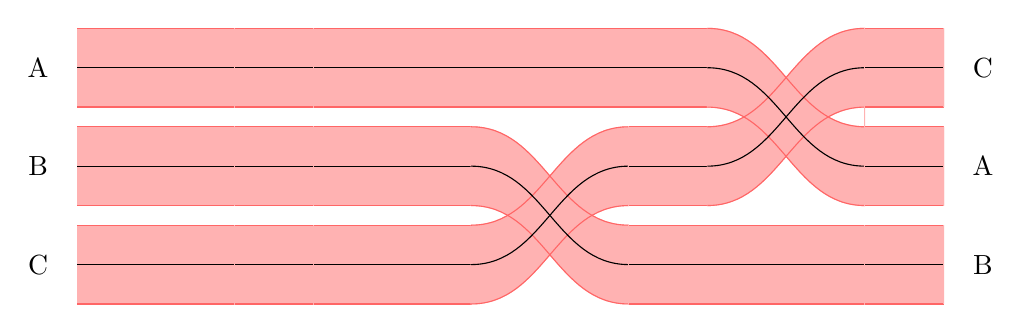
\begin{tikzpicture}[inner sep=0,outer sep=0]



 
\tape {0.000000} {2.500000} {1.000000} {1.000000}
\id{3}{0.000000}{3.000000}
\tape {0.000000} {1.250000} {1.000000} {1.000000}
\id{2}{0.000000}{1.750000}
\tape {1.000000} {2.500000} {0.000000} {1.000000}\draw (1.000000 , 3.000000) -- (1.000000 , 3.000000);
\tape {1.000000} {1.250000} {0.000000} {1.000000}\draw (1.000000 , 1.750000) -- (1.000000 , 1.750000);
\tape {1.000000} {2.500000} {1.000000} {1.000000}
\id{5}{1.000000}{3.000000}
\tape {1.000000} {1.250000} {1.000000} {1.000000}
\id{4}{1.000000}{1.750000}
\tape {2.000000} {2.500000} {0.000000} {1.000000}\draw (2.000000 , 3.000000) -- (2.000000 , 3.000000);
\tape {2.000000} {1.250000} {0.000000} {1.000000}\draw (2.000000 , 1.750000) -- (2.000000 , 1.750000);
\tape {0.000000} {0.000000} {1.000000} {1.000000}
\id{1}{0.000000}{0.500000}
\tape {2.000000} {2.500000} {0.000000} {1.000000}\draw (2.000000 , 3.000000) -- (2.000000 , 3.000000);
\tape {2.000000} {1.250000} {0.000000} {1.000000}\draw (2.000000 , 1.750000) -- (2.000000 , 1.750000);
\tape {1.000000} {0.000000} {1.000000} {1.000000}\draw (1.000000 , 0.500000) -- (2.000000 , 0.500000);
\tape {2.000000} {2.500000} {1.000000} {1.000000}
\id{8}{2.000000}{3.000000}
\tape {2.000000} {1.250000} {1.000000} {1.000000}
\id{7}{2.000000}{1.750000}
\tape {3.000000} {2.500000} {0.000000} {1.000000}\draw (3.000000 , 3.000000) -- (3.000000 , 3.000000);
\tape {3.000000} {1.250000} {0.000000} {1.000000}\draw (3.000000 , 1.750000) -- (3.000000 , 1.750000);
\tape {2.000000} {0.000000} {1.000000} {1.000000}
\id{6}{2.000000}{0.500000}
\tape {3.000000} {2.500000} {0.000000} {1.000000}\draw (3.000000 , 3.000000) -- (3.000000 , 3.000000);
\tape {3.000000} {1.250000} {0.000000} {1.000000}\draw (3.000000 , 1.750000) -- (3.000000 , 1.750000);
\tape {3.000000} {0.000000} {0.000000} {1.000000}\draw (3.000000 , 0.500000) -- (3.000000 , 0.500000);
\tape {3.000000} {2.500000} {1.000000} {1.000000}
\id{11}{3.000000}{3.000000}
\tape {3.000000} {1.250000} {1.000000} {1.000000}
\id{10}{3.000000}{1.750000}
\tape {4.000000} {2.500000} {0.000000} {1.000000}\draw (4.000000 , 3.000000) -- (4.000000 , 3.000000);
\tape {4.000000} {1.250000} {0.000000} {1.000000}\draw (4.000000 , 1.750000) -- (4.000000 , 1.750000);
\tape {3.000000} {0.000000} {1.000000} {1.000000}
\id{9}{3.000000}{0.500000}
\tape {4.000000} {2.500000} {0.000000} {1.000000}\draw (4.000000 , 3.000000) -- (4.000000 , 3.000000);
\tape {4.000000} {1.250000} {0.000000} {1.000000}\draw (4.000000 , 1.750000) -- (4.000000 , 1.750000);
\tape {4.000000} {0.000000} {0.000000} {1.000000}\draw (4.000000 , 0.500000) -- (4.000000 , 0.500000);
\tape {4.000000} {2.500000} {1.000000} {1.000000}
\id{16}{4.000000}{3.000000}
\tape {4.000000} {1.250000} {1.000000} {1.000000}
\id{13}{4.000000}{1.750000}
\tape {4.000000} {0.000000} {1.000000} {1.000000}
\id{12}{4.000000}{0.500000}
\tape {5.000000} {1.250000} {0.000000} {1.000000}\draw (5.000000 , 1.750000) -- (5.000000 , 1.750000);
\tape {5.000000} {0.000000} {0.000000} {1.000000}\draw (5.000000 , 0.500000) -- (5.000000 , 0.500000);
\swaptape {5.000000} {0.000000} {1} {1}\tape {7.000000} {1.250000} {1.000000} {1.000000}
\id{15}{7.000000}{1.750000}
\tape {7.000000} {0.000000} {1.000000} {1.000000}
\id{14}{7.000000}{0.500000}
\tape {8.000000} {1.250000} {0.000000} {1.000000}\draw (8.000000 , 1.750000) -- (8.000000 , 1.750000);
\tape {8.000000} {0.000000} {0.000000} {1.000000}\draw (8.000000 , 0.500000) -- (8.000000 , 0.500000);
\tape {5.000000} {2.500000} {3.000000} {1.000000}\draw (5.000000 , 3.000000) -- (8.000000 , 3.000000);
\tape {8.000000} {1.250000} {0.000000} {1.000000}\draw (8.000000 , 1.750000) -- (8.000000 , 1.750000);
\tape {8.000000} {0.000000} {0.000000} {1.000000}\draw (8.000000 , 0.500000) -- (8.000000 , 0.500000);
\swaptape {8.000000} {1.250000} {1} {1}\tape {8.000000} {0.000000} {1.000000} {1.000000}
\id{17}{8.000000}{0.500000}
\tape {10.000000} {2.250000} {0.000000} {1.000000}\draw (10.000000 , 1.250000) -- (10.000000 , 1.250000);
\tape {10.000000} {1.250000} {0.000000} {1.000000}\draw (10.000000 , 2.250000) -- (10.000000 , 2.250000);
\tape {9.000000} {0.000000} {1.000000} {1.000000}\draw (9.000000 , 0.500000) -- (10.000000 , 0.500000);
\tape {10.000000} {2.500000} {1.000000} {1.000000}
\id{20}{10.000000}{3.000000}
\tape {10.000000} {1.250000} {1.000000} {1.000000}
\id{19}{10.000000}{1.750000}
\tape {11.000000} {2.500000} {0.000000} {1.000000}\draw (11.000000 , 3.000000) -- (11.000000 , 3.000000);
\tape {11.000000} {1.250000} {0.000000} {1.000000}\draw (11.000000 , 1.750000) -- (11.000000 , 1.750000);
\tape {10.000000} {0.000000} {1.000000} {1.000000}
\id{18}{10.000000}{0.500000}
\tape {11.000000} {2.500000} {0.000000} {1.000000}\draw (11.000000 , 3.000000) -- (11.000000 , 3.000000);
\tape {11.000000} {1.250000} {0.000000} {1.000000}\draw (11.000000 , 1.750000) -- (11.000000 , 1.750000);
\tape {11.000000} {0.000000} {0.000000} {1.000000}\draw (11.000000 , 0.500000) -- (11.000000 , 0.500000);

\node () at (-0.500000, 3.000000) {A};
\node () at (-0.500000, 1.750000) {B};
\node () at (-0.500000, 0.500000) {C};
\node () at (11.500000, 3.000000) {C};
\node () at (11.500000, 1.750000) {A};
\node () at (11.500000, 0.500000) {B};


 \end{tikzpicture}

\end{document} 
